\sect{Berechnungsmodelle}

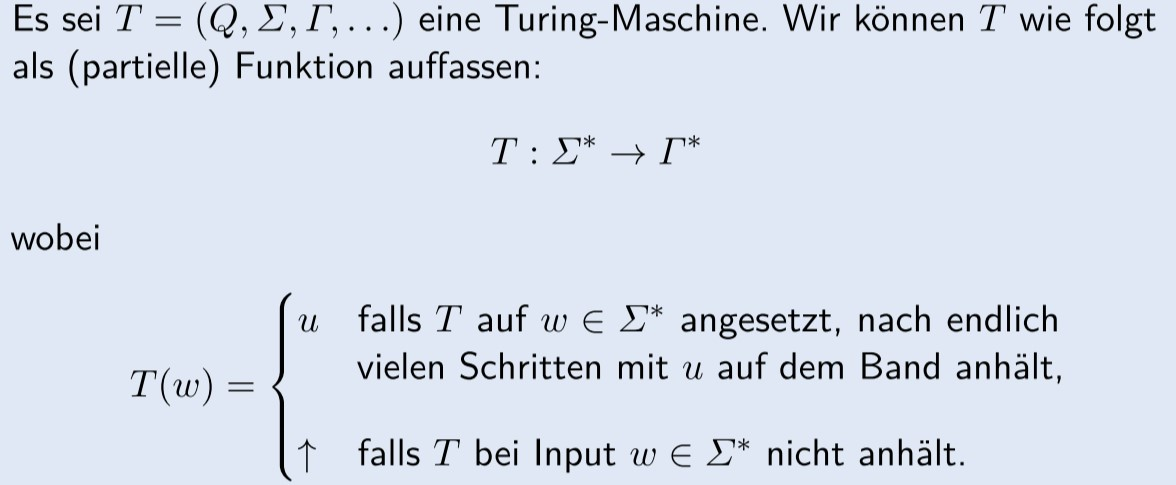
\includegraphics[scale=0.22]{turing-berechenbar-definition}

\ssect{Grundfunktionen}

Primitiv rekursiven Grundfunktionen:
\begin{itemize}
    \item $\forall n \in \N$ und jede Konstante $k \in \N$ die $n$-stellige \emph{konstante Funktion}\\ $c_k^n = \N^n \rightarrow \N$ mit $c_k^n (x_1, \dots, x_k) = k$
    \item Die \emph{Nachfolgerfunktion} $\eta: \N \rightarrow \N$ mit $\eta(x) = x + 1$
    \item $\forall n \in \N$ und jedes $1 < k < n$ die $n$-stellige \emph{Projektion} auf die $k$-te Komponente $\pi_k^n = \N^n \rightarrow \N$ mit $\pi_k^n (x_1, \dots, x_k, \dots, x_n) = k$
\end{itemize}

\sssect{Loop (Primitiv-Rekursiv)}

\begin{itemize}
    \item Zuweisungen: $x = y + c$ und $x = y - c$
    \item Sequenzen: $P$ und $Q \rightarrow P;Q$
    \item Schleifen: $P \rightarrow$ \texttt{Loop} $x$ \texttt{Do} $P$ \texttt{End}
\end{itemize}

\textbf{Beispiele:}

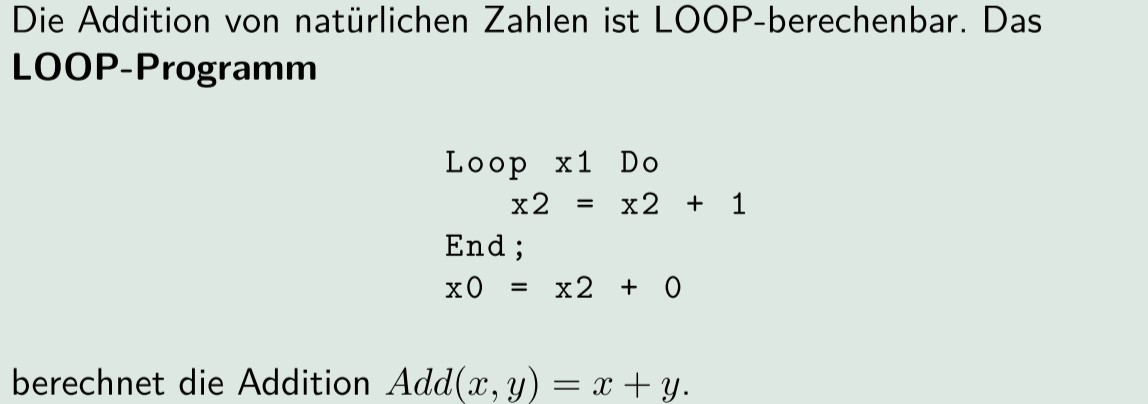
\includegraphics[scale=0.22]{addition-loop}

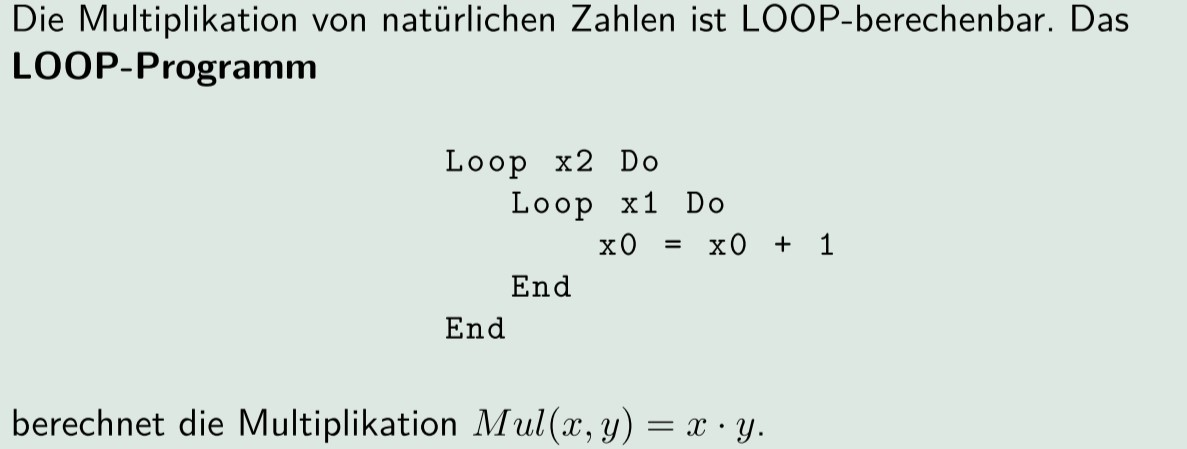
\includegraphics[scale=0.215]{multiplikation-loop}

\columnbreak

\sssect{While (Turing-complete)}

Erweiterung der Sprache \texttt{Loop} um\\
\texttt{While} $x_i > 0$ \texttt{Do} $\dots$ \texttt{End}
\begin{itemize}
    \item Jedes \texttt{Loop}-Programm ist auch ein \texttt{While}-Programm
    \item \texttt{While}-Programme terminieren nicht immer (Endlos-Schleife)
\end{itemize}

\sssect{GOTO (Turing-complete)}

\begin{itemize}
    \item Zuweisungen:\\
    $\texttt{Mk}: x_i = x_j + c$ \\
    $\texttt{Mk}: x_i = x_j - c$
    \item Sprunganweisung:\\
    \texttt{Mk}: \texttt{If} $x_i = c$ \texttt{Then Goto Mr} \\
    \texttt{Mk}: \texttt{Goto Mr}
    \item Halt-Anweisung:\\
    \texttt{Mk:} \texttt{HALT}
\end{itemize}

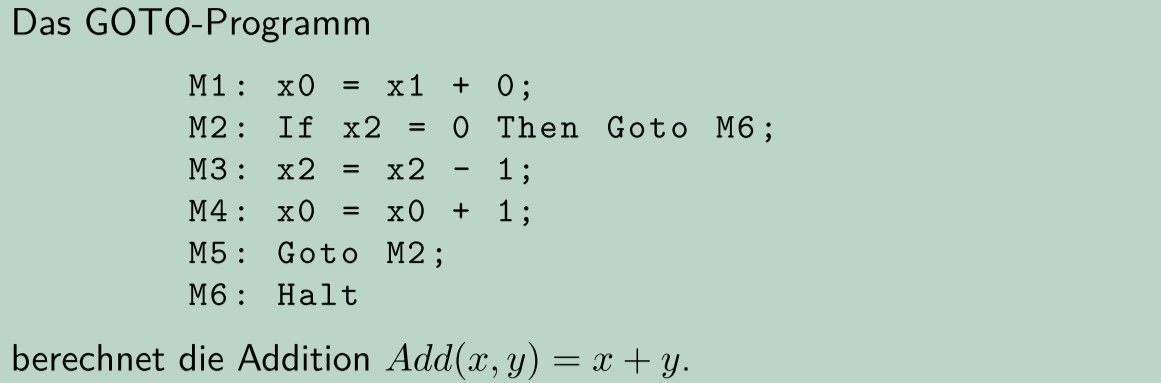
\includegraphics[scale=0.22]{addition-goto}%